\htmlhr
\section{Interning checker\label{interning-checker}}

If the Interning checker issues no warnings for a given program, then all
reference equality tests (i.e., ``\code{==}'') in that program operate on
interned types.  
Interning is a design pattern in which the same object is used whenever two
different objects would be considered equal.  Interning is also known as
canonicalization or hash-consing, and it is related to the flyweight design
pattern.
Interning can save memory and can speed up testing for
equality by permitting use of \code{==}; however, use of \code{==} on
non-interned values can result in subtle bugs.  For example:

\begin{Verbatim}
  Integer x = new Integer(22);
  Integer y = new Integer(22);
  System.out.println(x == y);  // prints false!
\end{Verbatim}

The Interning checker helps programmers to prevent such bugs.
The Interning checker also helps to prevent performance problems that result
from failure to use interning.
(See Section~\ref{checker-guarantees} for caveats to the checker's guarantees.)


\subsection{Interning annotations\label{interning-annotations}}

Two qualifiers are part of the Interning type system.

\begin{description}

\item[\code{@\refclass{interning/quals}{Interned}}]
  indicates a type that includes only interned values (no non-interned
  values).

\item[\<@\refclass{interning/quals}{PolyInterned}>]
  indicates qualifier polymorphism.  For a description of
  \<@\refclass{interning/quals}{PolyInterned}>, see
  Section~\ref{qualifier-polymorphism}.

\end{description}


\subsection{Annotating your code with \code{@Interned}\label{annotating-with-interned}}

\begin{figure}
\begin{center}
\resizebox{!}{2.5cm}{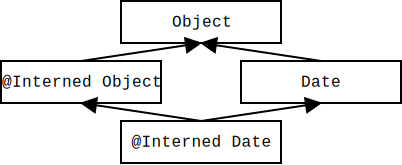
\includegraphics{figures/interning}}
\end{center}
%BEGIN LATEX
\vspace{-1.5\baselineskip}
%END LATEX
\caption{Type hierarchy for the Interning type system.}
\label{fig:interning-hierarchy}
\end{figure}

In order to perform checking, you must annotate your code with the \code{@\refclass{interning/quals}{Interned}}
type annotation, which indicates a type for the canonical representation of an
object:

\begin{Verbatim}
            String s1 = ...;  // type is (uninterned) "String"
  @Interned String s2 = ...;  // Java type is "String", but checker treats it as "Interned String"
\end{Verbatim}

The type system enforced by the checker plugin ensures that only interned
values can be assigned to \code{s2}.

To specify that \emph{all} objects of a given type are interned, annotate the
class declaration:

\begin{Verbatim}
  public @Interned class MyInternedClass { ... }
\end{Verbatim}

This is equivalent to annotating every use of \code{MyInternedClass}, in a
declaration or elsewhere.  For example, \code{enum} classes are implicitly
so annotated.


\subsubsection{Implicit qualifiers\label{interning-implicit-qualifiers}}

As described in Section~\ref{effective-qualifier}, the Interning checker
adds implicit qualifiers, reducing the number of annotations that must
appear in your code.
For example, String literals and the null literal are always considered interned, and
object creation expressions (using \code{new}) are never considered
\code{@\refclass{interning/quals}{Interned}} unless they are annotated as such, as in

%BEGIN LATEX
\begin{smaller}
%END LATEX
\begin{Verbatim}
@Interned Double internedDoubleZero = new @Interned Double(0); // canonical representation for Double zero
\end{Verbatim}
%BEGIN LATEX
\end{smaller}
%END LATEX

For a complete description of all implicit interning qualifiers, see the
Javadoc for \refclass{interning}{InterningAnnotatedTypeFactory}.


\subsection{What the Interning checker checks\label{interning-checks}}

Objects of an \code{@\refclass{interning/quals}{Interned}} type may be safely compared using the ``\code{==}''
operator.

The checker issues a warning in two cases:

\begin{enumerate}

\item
  When a reference (in)equality operator (``\code{==}'' or ``\code{!=}'')
  has an operand of non-\code{@\refclass{interning/quals}{Interned}} type.

\item
  When a non-\code{@\refclass{interning/quals}{Interned}} type is used where an \code{@\refclass{interning/quals}{Interned}} type
  is expected.

\end{enumerate}

This example shows both sorts of problems:

\begin{Verbatim}
            Object  obj;
  @Interned Object iobj;
  ...
  if (obj == iobj) { ... }  // checker warning: reference equality test is unsafe
  iobj = obj;               // checker warning: iobj's referent may no longer be interned
\end{Verbatim}

The checker also issues a warning when \code{.equals} is used where
\code{==} could be safely used.  You can disable this behavior via the
javac \code{-Alint} command-line option, like so: \code{-Alint=-dotequals}.

For a complete description of all checks performed by
  the checker, see the Javadoc for
  \refclass{interning}{InterningVisitor}.


\subsection{Examples\label{interning-example}}

To try the Interning checker on a source file that uses the \code{@\refclass{interning/quals}{Interned}} qualifier,
use the following command (where \code{javac} is the JSR 308 compiler that
is distributed with the Checker Framework):

\begin{Verbatim}
  javac -processor checkers.interning.InterningChecker examples/InterningExample.java
\end{Verbatim}

\noindent
Compilation will complete without warnings.

To see the checker warn about incorrect usage of annotations, use the following
command:

\begin{Verbatim}
  javac -processor checkers.interning.InterningChecker examples/InterningExampleWithWarnings.java
\end{Verbatim}

\noindent
The compiler will issue a warning regarding violation of the semantics of
\code{@\refclass{interning/quals}{Interned}}.
% in the \code{InterningExampleWithWarnings.java} file.


The Daikon invariant detector
(\myurl{http://groups.csail.mit.edu/pag/daikon/}) is also annotated with
\code{@\refclass{interning/quals}{Interned}}.  From directory \code{java},
run \code{make check-interning}.



% LocalWords:  plugin MyInternedClass enum InterningExampleWithWarnings java
% LocalWords:  PolyInterned Alint dotequals quals InterningAnnotatedTypeFactory
% LocalWords:  javac InterningVisitor
